% Created by tikzDevice version 0.12.6 on 2024-04-23 11:24:49
% !TEX encoding = UTF-8 Unicode
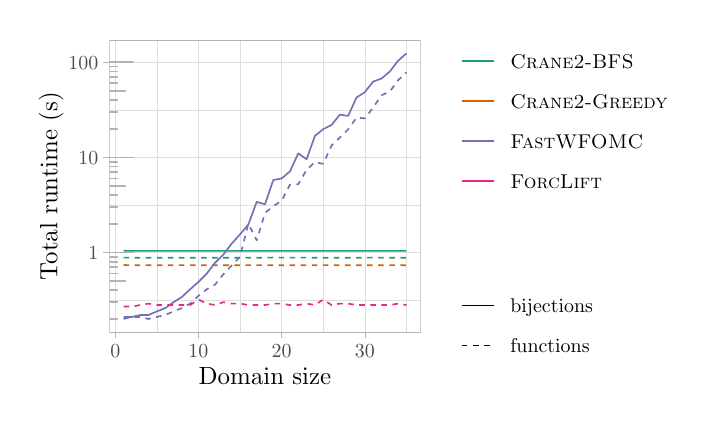
\begin{tikzpicture}[x=1pt,y=1pt]
\definecolor{fillColor}{RGB}{255,255,255}
\path[use as bounding box,fill=fillColor,fill opacity=0.00] (0,0) rectangle (240.29,135.16);
\begin{scope}
\path[clip] (  0.00,  0.00) rectangle (240.29,135.16);
\definecolor{drawColor}{RGB}{255,255,255}
\definecolor{fillColor}{RGB}{255,255,255}

\path[draw=drawColor,line width= 0.5pt,line join=round,line cap=round,fill=fillColor] (  0.00,  0.00) rectangle (240.29,135.16);
\end{scope}
\begin{scope}
\path[clip] ( 29.55, 25.11) rectangle (141.96,130.66);
\definecolor{fillColor}{RGB}{255,255,255}

\path[fill=fillColor] ( 29.55, 25.11) rectangle (141.96,130.66);
\definecolor{drawColor}{gray}{0.87}

\path[draw=drawColor,line width= 0.1pt,line join=round] ( 29.55, 36.74) --
	(141.96, 36.74);

\path[draw=drawColor,line width= 0.1pt,line join=round] ( 29.55, 71.11) --
	(141.96, 71.11);

\path[draw=drawColor,line width= 0.1pt,line join=round] ( 29.55,105.49) --
	(141.96,105.49);

\path[draw=drawColor,line width= 0.1pt,line join=round] ( 46.68, 25.11) --
	( 46.68,130.66);

\path[draw=drawColor,line width= 0.1pt,line join=round] ( 76.74, 25.11) --
	( 76.74,130.66);

\path[draw=drawColor,line width= 0.1pt,line join=round] (106.80, 25.11) --
	(106.80,130.66);

\path[draw=drawColor,line width= 0.1pt,line join=round] (136.85, 25.11) --
	(136.85,130.66);

\path[draw=drawColor,line width= 0.2pt,line join=round] ( 29.55, 53.93) --
	(141.96, 53.93);

\path[draw=drawColor,line width= 0.2pt,line join=round] ( 29.55, 88.30) --
	(141.96, 88.30);

\path[draw=drawColor,line width= 0.2pt,line join=round] ( 29.55,122.67) --
	(141.96,122.67);

\path[draw=drawColor,line width= 0.2pt,line join=round] ( 31.65, 25.11) --
	( 31.65,130.66);

\path[draw=drawColor,line width= 0.2pt,line join=round] ( 61.71, 25.11) --
	( 61.71,130.66);

\path[draw=drawColor,line width= 0.2pt,line join=round] ( 91.77, 25.11) --
	( 91.77,130.66);

\path[draw=drawColor,line width= 0.2pt,line join=round] (121.82, 25.11) --
	(121.82,130.66);
\definecolor{drawColor}{RGB}{27,158,119}

\path[draw=drawColor,line width= 0.6pt,line join=round] ( 34.66, 54.53) --
	( 37.66, 54.50) --
	( 40.67, 54.50) --
	( 43.67, 54.49) --
	( 46.68, 54.49) --
	( 49.68, 54.49) --
	( 52.69, 54.49) --
	( 55.70, 54.50) --
	( 58.70, 54.50) --
	( 61.71, 54.49) --
	( 64.71, 54.49) --
	( 67.72, 54.49) --
	( 70.73, 54.49) --
	( 73.73, 54.49) --
	( 76.74, 54.50) --
	( 79.74, 54.50) --
	( 82.75, 54.50) --
	( 85.75, 54.50) --
	( 88.76, 54.49) --
	( 91.77, 54.50) --
	( 94.77, 54.50) --
	( 97.78, 54.49) --
	(100.78, 54.50) --
	(103.79, 54.50) --
	(106.80, 54.50) --
	(109.80, 54.50) --
	(112.81, 54.49) --
	(115.81, 54.50) --
	(118.82, 54.50) --
	(121.82, 54.50) --
	(124.83, 54.50) --
	(127.84, 54.50) --
	(130.84, 54.50) --
	(133.85, 54.50) --
	(136.85, 54.50);

\path[draw=drawColor,line width= 0.6pt,dash pattern=on 2pt off 2pt ,line join=round] ( 34.66, 52.07) --
	( 37.66, 52.04) --
	( 40.67, 52.04) --
	( 43.67, 52.04) --
	( 46.68, 52.04) --
	( 49.68, 52.05) --
	( 52.69, 52.04) --
	( 55.70, 52.05) --
	( 58.70, 52.04) --
	( 61.71, 52.04) --
	( 64.71, 52.04) --
	( 67.72, 52.04) --
	( 70.73, 52.04) --
	( 73.73, 52.04) --
	( 76.74, 52.05) --
	( 79.74, 52.05) --
	( 82.75, 52.04) --
	( 85.75, 52.04) --
	( 88.76, 52.09) --
	( 91.77, 52.05) --
	( 94.77, 52.05) --
	( 97.78, 52.05) --
	(100.78, 52.05) --
	(103.79, 52.04) --
	(106.80, 52.04) --
	(109.80, 52.04) --
	(112.81, 52.04) --
	(115.81, 52.04) --
	(118.82, 52.04) --
	(121.82, 52.05) --
	(124.83, 52.05) --
	(127.84, 52.05) --
	(130.84, 52.04) --
	(133.85, 52.05) --
	(136.85, 52.04);
\definecolor{drawColor}{RGB}{217,95,2}

\path[draw=drawColor,line width= 0.6pt,dash pattern=on 2pt off 2pt ,line join=round] ( 34.66, 49.39) --
	( 37.66, 49.33) --
	( 40.67, 49.33) --
	( 43.67, 49.33) --
	( 46.68, 49.33) --
	( 49.68, 49.33) --
	( 52.69, 49.33) --
	( 55.70, 49.35) --
	( 58.70, 49.35) --
	( 61.71, 49.33) --
	( 64.71, 49.33) --
	( 67.72, 49.33) --
	( 70.73, 49.33) --
	( 73.73, 49.33) --
	( 76.74, 49.33) --
	( 79.74, 49.35) --
	( 82.75, 49.35) --
	( 85.75, 49.35) --
	( 88.76, 49.33) --
	( 91.77, 49.33) --
	( 94.77, 49.33) --
	( 97.78, 49.33) --
	(100.78, 49.33) --
	(103.79, 49.33) --
	(106.80, 49.35) --
	(109.80, 49.35) --
	(112.81, 49.33) --
	(115.81, 49.33) --
	(118.82, 49.33) --
	(121.82, 49.33) --
	(124.83, 49.33) --
	(127.84, 49.33) --
	(130.84, 49.35) --
	(133.85, 49.35) --
	(136.85, 49.33);
\definecolor{drawColor}{RGB}{117,112,179}

\path[draw=drawColor,line width= 0.6pt,line join=round] ( 34.66, 30.63) --
	( 37.66, 30.63) --
	( 40.67, 31.33) --
	( 43.67, 31.33) --
	( 46.68, 32.63) --
	( 49.68, 33.82) --
	( 52.69, 35.96) --
	( 55.70, 37.83) --
	( 58.70, 40.62) --
	( 61.71, 43.28) --
	( 64.71, 46.30) --
	( 67.72, 50.22) --
	( 70.73, 53.16) --
	( 73.73, 57.14) --
	( 76.74, 60.47) --
	( 79.74, 64.05) --
	( 82.75, 72.20) --
	( 85.75, 71.34) --
	( 88.76, 80.12) --
	( 91.77, 80.67) --
	( 94.77, 83.21) --
	( 97.78, 89.74) --
	(100.78, 87.61) --
	(103.79, 96.04) --
	(106.80, 98.47) --
	(109.80, 99.99) --
	(112.81,103.72) --
	(115.81,103.27) --
	(118.82,109.92) --
	(121.82,111.85) --
	(124.83,115.67) --
	(127.84,116.78) --
	(130.84,119.28) --
	(133.85,123.20) --
	(136.85,125.87);

\path[draw=drawColor,line width= 0.6pt,dash pattern=on 2pt off 2pt ,line join=round] ( 34.66, 29.90) --
	( 37.66, 30.63) --
	( 40.67, 30.63) --
	( 43.67, 29.90) --
	( 46.68, 30.63) --
	( 49.68, 31.33) --
	( 52.69, 32.63) --
	( 55.70, 33.82) --
	( 58.70, 35.45) --
	( 61.71, 38.26) --
	( 64.71, 40.62) --
	( 67.72, 42.34) --
	( 70.73, 46.05) --
	( 73.73, 49.23) --
	( 76.74, 52.36) --
	( 79.74, 64.35) --
	( 82.75, 58.30) --
	( 85.75, 68.19) --
	( 88.76, 70.67) --
	( 91.77, 72.59) --
	( 94.77, 78.45) --
	( 97.78, 78.57) --
	(100.78, 83.81) --
	(103.79, 86.56) --
	(106.80, 85.94) --
	(109.80, 92.57) --
	(112.81, 95.46) --
	(115.81, 98.41) --
	(118.82,102.64) --
	(121.82,102.38) --
	(124.83,106.28) --
	(127.84,110.72) --
	(130.84,112.06) --
	(133.85,116.16) --
	(136.85,119.03);
\definecolor{drawColor}{RGB}{231,41,138}

\path[draw=drawColor,line width= 0.6pt,dash pattern=on 2pt off 2pt ,line join=round] ( 34.66, 34.38) --
	( 37.66, 34.38) --
	( 40.67, 34.93) --
	( 43.67, 35.45) --
	( 46.68, 34.93) --
	( 49.68, 34.93) --
	( 52.69, 34.93) --
	( 55.70, 34.93) --
	( 58.70, 34.93) --
	( 61.71, 36.92) --
	( 64.71, 35.45) --
	( 67.72, 34.93) --
	( 70.73, 35.96) --
	( 73.73, 35.45) --
	( 76.74, 35.45) --
	( 79.74, 34.93) --
	( 82.75, 34.93) --
	( 85.75, 34.93) --
	( 88.76, 35.45) --
	( 91.77, 35.45) --
	( 94.77, 34.93) --
	( 97.78, 34.93) --
	(100.78, 35.45) --
	(103.79, 34.93) --
	(106.80, 36.92) --
	(109.80, 34.93) --
	(112.81, 35.45) --
	(115.81, 35.45) --
	(118.82, 34.93) --
	(121.82, 34.93) --
	(124.83, 34.93) --
	(127.84, 34.93) --
	(130.84, 34.93) --
	(133.85, 35.45) --
	(136.85, 34.93);
\definecolor{drawColor}{gray}{0.70}

\path[draw=drawColor,line width= 0.6pt,line join=round,line cap=round] ( 29.55, 29.90) -- ( 32.39, 29.90);

\path[draw=drawColor,line width= 0.6pt,line join=round,line cap=round] ( 29.55, 35.96) -- ( 32.39, 35.96);

\path[draw=drawColor,line width= 0.6pt,line join=round,line cap=round] ( 29.55, 40.25) -- ( 32.39, 40.25);

\path[draw=drawColor,line width= 0.6pt,line join=round,line cap=round] ( 29.55, 43.58) -- ( 35.24, 43.58);

\path[draw=drawColor,line width= 0.6pt,line join=round,line cap=round] ( 29.55, 46.30) -- ( 32.39, 46.30);

\path[draw=drawColor,line width= 0.6pt,line join=round,line cap=round] ( 29.55, 48.60) -- ( 32.39, 48.60);

\path[draw=drawColor,line width= 0.6pt,line join=round,line cap=round] ( 29.55, 50.60) -- ( 32.39, 50.60);

\path[draw=drawColor,line width= 0.6pt,line join=round,line cap=round] ( 29.55, 52.36) -- ( 32.39, 52.36);

\path[draw=drawColor,line width= 0.6pt,line join=round,line cap=round] ( 29.55, 53.93) -- ( 38.08, 53.93);

\path[draw=drawColor,line width= 0.6pt,line join=round,line cap=round] ( 29.55, 64.28) -- ( 32.39, 64.28);

\path[draw=drawColor,line width= 0.6pt,line join=round,line cap=round] ( 29.55, 70.33) -- ( 32.39, 70.33);

\path[draw=drawColor,line width= 0.6pt,line join=round,line cap=round] ( 29.55, 74.62) -- ( 32.39, 74.62);

\path[draw=drawColor,line width= 0.6pt,line join=round,line cap=round] ( 29.55, 77.95) -- ( 35.24, 77.95);

\path[draw=drawColor,line width= 0.6pt,line join=round,line cap=round] ( 29.55, 80.67) -- ( 32.39, 80.67);

\path[draw=drawColor,line width= 0.6pt,line join=round,line cap=round] ( 29.55, 82.98) -- ( 32.39, 82.98);

\path[draw=drawColor,line width= 0.6pt,line join=round,line cap=round] ( 29.55, 84.97) -- ( 32.39, 84.97);

\path[draw=drawColor,line width= 0.6pt,line join=round,line cap=round] ( 29.55, 86.73) -- ( 32.39, 86.73);

\path[draw=drawColor,line width= 0.6pt,line join=round,line cap=round] ( 29.55, 88.30) -- ( 38.08, 88.30);

\path[draw=drawColor,line width= 0.6pt,line join=round,line cap=round] ( 29.55, 98.65) -- ( 32.39, 98.65);

\path[draw=drawColor,line width= 0.6pt,line join=round,line cap=round] ( 29.55,104.70) -- ( 32.39,104.70);

\path[draw=drawColor,line width= 0.6pt,line join=round,line cap=round] ( 29.55,108.99) -- ( 32.39,108.99);

\path[draw=drawColor,line width= 0.6pt,line join=round,line cap=round] ( 29.55,112.32) -- ( 35.24,112.32);

\path[draw=drawColor,line width= 0.6pt,line join=round,line cap=round] ( 29.55,115.05) -- ( 32.39,115.05);

\path[draw=drawColor,line width= 0.6pt,line join=round,line cap=round] ( 29.55,117.35) -- ( 32.39,117.35);

\path[draw=drawColor,line width= 0.6pt,line join=round,line cap=round] ( 29.55,119.34) -- ( 32.39,119.34);

\path[draw=drawColor,line width= 0.6pt,line join=round,line cap=round] ( 29.55,121.10) -- ( 32.39,121.10);

\path[draw=drawColor,line width= 0.6pt,line join=round,line cap=round] ( 29.55,122.67) -- ( 38.08,122.67);

\path[draw=drawColor,line width= 0.5pt,line join=round,line cap=round] ( 29.55, 25.11) rectangle (141.96,130.66);
\end{scope}
\begin{scope}
\path[clip] (  0.00,  0.00) rectangle (240.29,135.16);
\definecolor{drawColor}{gray}{0.30}

\node[text=drawColor,anchor=base east,inner sep=0pt, outer sep=0pt, scale=  0.72] at ( 25.50, 51.45) {1};

\node[text=drawColor,anchor=base east,inner sep=0pt, outer sep=0pt, scale=  0.72] at ( 25.50, 85.82) {10};

\node[text=drawColor,anchor=base east,inner sep=0pt, outer sep=0pt, scale=  0.72] at ( 25.50,120.19) {100};
\end{scope}
\begin{scope}
\path[clip] (  0.00,  0.00) rectangle (240.29,135.16);
\definecolor{drawColor}{gray}{0.70}

\path[draw=drawColor,line width= 0.2pt,line join=round] ( 27.30, 53.93) --
	( 29.55, 53.93);

\path[draw=drawColor,line width= 0.2pt,line join=round] ( 27.30, 88.30) --
	( 29.55, 88.30);

\path[draw=drawColor,line width= 0.2pt,line join=round] ( 27.30,122.67) --
	( 29.55,122.67);
\end{scope}
\begin{scope}
\path[clip] (  0.00,  0.00) rectangle (240.29,135.16);
\definecolor{drawColor}{gray}{0.70}

\path[draw=drawColor,line width= 0.2pt,line join=round] ( 31.65, 22.86) --
	( 31.65, 25.11);

\path[draw=drawColor,line width= 0.2pt,line join=round] ( 61.71, 22.86) --
	( 61.71, 25.11);

\path[draw=drawColor,line width= 0.2pt,line join=round] ( 91.77, 22.86) --
	( 91.77, 25.11);

\path[draw=drawColor,line width= 0.2pt,line join=round] (121.82, 22.86) --
	(121.82, 25.11);
\end{scope}
\begin{scope}
\path[clip] (  0.00,  0.00) rectangle (240.29,135.16);
\definecolor{drawColor}{gray}{0.30}

\node[text=drawColor,anchor=base,inner sep=0pt, outer sep=0pt, scale=  0.72] at ( 31.65, 16.10) {0};

\node[text=drawColor,anchor=base,inner sep=0pt, outer sep=0pt, scale=  0.72] at ( 61.71, 16.10) {10};

\node[text=drawColor,anchor=base,inner sep=0pt, outer sep=0pt, scale=  0.72] at ( 91.77, 16.10) {20};

\node[text=drawColor,anchor=base,inner sep=0pt, outer sep=0pt, scale=  0.72] at (121.82, 16.10) {30};
\end{scope}
\begin{scope}
\path[clip] (  0.00,  0.00) rectangle (240.29,135.16);
\definecolor{drawColor}{RGB}{0,0,0}

\node[text=drawColor,anchor=base,inner sep=0pt, outer sep=0pt, scale=  0.90] at ( 85.75,  6.25) {Domain size};
\end{scope}
\begin{scope}
\path[clip] (  0.00,  0.00) rectangle (240.29,135.16);
\definecolor{drawColor}{RGB}{0,0,0}

\node[text=drawColor,rotate= 90.00,anchor=base,inner sep=0pt, outer sep=0pt, scale=  0.90] at ( 10.70, 77.89) {Total runtime (s)};
\end{scope}
\begin{scope}
\path[clip] (  0.00,  0.00) rectangle (240.29,135.16);
\definecolor{fillColor}{RGB}{255,255,255}

\path[fill=fillColor] (150.96, 67.93) rectangle (235.79,147.20);
\end{scope}
\begin{scope}
\path[clip] (  0.00,  0.00) rectangle (240.29,135.16);
\definecolor{fillColor}{RGB}{255,255,255}

\path[fill=fillColor] (155.46,115.79) rectangle (169.92,130.25);
\end{scope}
\begin{scope}
\path[clip] (  0.00,  0.00) rectangle (240.29,135.16);
\definecolor{drawColor}{RGB}{27,158,119}

\path[draw=drawColor,line width= 0.6pt,line join=round] (156.91,123.02) -- (168.47,123.02);
\end{scope}
\begin{scope}
\path[clip] (  0.00,  0.00) rectangle (240.29,135.16);
\definecolor{fillColor}{RGB}{255,255,255}

\path[fill=fillColor] (155.46,101.34) rectangle (169.92,115.79);
\end{scope}
\begin{scope}
\path[clip] (  0.00,  0.00) rectangle (240.29,135.16);
\definecolor{drawColor}{RGB}{217,95,2}

\path[draw=drawColor,line width= 0.6pt,line join=round] (156.91,108.57) -- (168.47,108.57);
\end{scope}
\begin{scope}
\path[clip] (  0.00,  0.00) rectangle (240.29,135.16);
\definecolor{fillColor}{RGB}{255,255,255}

\path[fill=fillColor] (155.46, 86.89) rectangle (169.92,101.34);
\end{scope}
\begin{scope}
\path[clip] (  0.00,  0.00) rectangle (240.29,135.16);
\definecolor{drawColor}{RGB}{117,112,179}

\path[draw=drawColor,line width= 0.6pt,line join=round] (156.91, 94.11) -- (168.47, 94.11);
\end{scope}
\begin{scope}
\path[clip] (  0.00,  0.00) rectangle (240.29,135.16);
\definecolor{fillColor}{RGB}{255,255,255}

\path[fill=fillColor] (155.46, 72.43) rectangle (169.92, 86.89);
\end{scope}
\begin{scope}
\path[clip] (  0.00,  0.00) rectangle (240.29,135.16);
\definecolor{drawColor}{RGB}{231,41,138}

\path[draw=drawColor,line width= 0.6pt,line join=round] (156.91, 79.66) -- (168.47, 79.66);
\end{scope}
\begin{scope}
\path[clip] (  0.00,  0.00) rectangle (240.29,135.16);
\definecolor{drawColor}{RGB}{0,0,0}

\node[text=drawColor,anchor=base west,inner sep=0pt, outer sep=0pt, scale=  0.72] at (174.42,120.54) {\textsc{Crane2-BFS}};
\end{scope}
\begin{scope}
\path[clip] (  0.00,  0.00) rectangle (240.29,135.16);
\definecolor{drawColor}{RGB}{0,0,0}

\node[text=drawColor,anchor=base west,inner sep=0pt, outer sep=0pt, scale=  0.72] at (174.42,106.09) {\textsc{Crane2-Greedy}};
\end{scope}
\begin{scope}
\path[clip] (  0.00,  0.00) rectangle (240.29,135.16);
\definecolor{drawColor}{RGB}{0,0,0}

\node[text=drawColor,anchor=base west,inner sep=0pt, outer sep=0pt, scale=  0.72] at (174.42, 91.63) {\textsc{FastWFOMC}};
\end{scope}
\begin{scope}
\path[clip] (  0.00,  0.00) rectangle (240.29,135.16);
\definecolor{drawColor}{RGB}{0,0,0}

\node[text=drawColor,anchor=base west,inner sep=0pt, outer sep=0pt, scale=  0.72] at (174.42, 77.18) {\textsc{ForcLift}};
\end{scope}
\begin{scope}
\path[clip] (  0.00,  0.00) rectangle (240.29,135.16);
\definecolor{fillColor}{RGB}{255,255,255}

\path[fill=fillColor] (150.96,  8.58) rectangle (208.75, 58.93);
\end{scope}
\begin{scope}
\path[clip] (  0.00,  0.00) rectangle (240.29,135.16);
\definecolor{fillColor}{RGB}{255,255,255}

\path[fill=fillColor] (155.46, 27.53) rectangle (169.92, 41.98);
\end{scope}
\begin{scope}
\path[clip] (  0.00,  0.00) rectangle (240.29,135.16);
\definecolor{drawColor}{RGB}{0,0,0}

\path[draw=drawColor,line width= 0.6pt,line join=round] (156.91, 34.76) -- (168.47, 34.76);
\end{scope}
\begin{scope}
\path[clip] (  0.00,  0.00) rectangle (240.29,135.16);
\definecolor{fillColor}{RGB}{255,255,255}

\path[fill=fillColor] (155.46, 13.08) rectangle (169.92, 27.53);
\end{scope}
\begin{scope}
\path[clip] (  0.00,  0.00) rectangle (240.29,135.16);
\definecolor{drawColor}{RGB}{0,0,0}

\path[draw=drawColor,line width= 0.6pt,dash pattern=on 2pt off 2pt ,line join=round] (156.91, 20.30) -- (168.47, 20.30);
\end{scope}
\begin{scope}
\path[clip] (  0.00,  0.00) rectangle (240.29,135.16);
\definecolor{drawColor}{RGB}{0,0,0}

\node[text=drawColor,anchor=base west,inner sep=0pt, outer sep=0pt, scale=  0.72] at (174.42, 32.28) {bijections};
\end{scope}
\begin{scope}
\path[clip] (  0.00,  0.00) rectangle (240.29,135.16);
\definecolor{drawColor}{RGB}{0,0,0}

\node[text=drawColor,anchor=base west,inner sep=0pt, outer sep=0pt, scale=  0.72] at (174.42, 17.82) {functions};
\end{scope}
\end{tikzpicture}
